

\documentclass[12pt]{article}\usepackage[]{graphicx}\usepackage[]{color}
%% maxwidth is the original width if it is less than linewidth
%% otherwise use linewidth (to make sure the graphics do not exceed the margin)
\makeatletter
\def\maxwidth{ %
  \ifdim\Gin@nat@width>\linewidth
    \linewidth
  \else
    \Gin@nat@width
  \fi
}
\makeatother

\definecolor{fgcolor}{rgb}{0.345, 0.345, 0.345}
\newcommand{\hlnum}[1]{\textcolor[rgb]{0.686,0.059,0.569}{#1}}%
\newcommand{\hlstr}[1]{\textcolor[rgb]{0.192,0.494,0.8}{#1}}%
\newcommand{\hlcom}[1]{\textcolor[rgb]{0.678,0.584,0.686}{\textit{#1}}}%
\newcommand{\hlopt}[1]{\textcolor[rgb]{0,0,0}{#1}}%
\newcommand{\hlstd}[1]{\textcolor[rgb]{0.345,0.345,0.345}{#1}}%
\newcommand{\hlkwa}[1]{\textcolor[rgb]{0.161,0.373,0.58}{\textbf{#1}}}%
\newcommand{\hlkwb}[1]{\textcolor[rgb]{0.69,0.353,0.396}{#1}}%
\newcommand{\hlkwc}[1]{\textcolor[rgb]{0.333,0.667,0.333}{#1}}%
\newcommand{\hlkwd}[1]{\textcolor[rgb]{0.737,0.353,0.396}{\textbf{#1}}}%
\let\hlipl\hlkwb

\usepackage{framed}
\makeatletter
\newenvironment{kframe}{%
 \def\at@end@of@kframe{}%
 \ifinner\ifhmode%
  \def\at@end@of@kframe{\end{minipage}}%
  \begin{minipage}{\columnwidth}%
 \fi\fi%
 \def\FrameCommand##1{\hskip\@totalleftmargin \hskip-\fboxsep
 \colorbox{shadecolor}{##1}\hskip-\fboxsep
     % There is no \\@totalrightmargin, so:
     \hskip-\linewidth \hskip-\@totalleftmargin \hskip\columnwidth}%
 \MakeFramed {\advance\hsize-\width
   \@totalleftmargin\z@ \linewidth\hsize
   \@setminipage}}%
 {\par\unskip\endMakeFramed%
 \at@end@of@kframe}
\makeatother

\definecolor{shadecolor}{rgb}{.97, .97, .97}
\definecolor{messagecolor}{rgb}{0, 0, 0}
\definecolor{warningcolor}{rgb}{1, 0, 1}
\definecolor{errorcolor}{rgb}{1, 0, 0}
\newenvironment{knitrout}{}{} % an empty environment to be redefined in TeX

\usepackage{alltt}
\usepackage{geometry}
\usepackage{graphicx,amsmath,enumerate, amssymb, multirow, anysize, booktabs, threeparttable, amsfonts, bbm, dcolumn}
\usepackage{setspace,listings,dsfont}
% \usepackage[square, numbers, sort]{natbib}
\usepackage{natbib}
\usepackage{color,soul}
\usepackage{fancyhdr}
\usepackage{graphicx}
\usepackage{placeins}
\usepackage{titlesec}
\usepackage{setspace,float,lscape,subfigure,amsmath,multirow,color}
\usepackage[font=small,format=hang,labelfont=bf,up,textfont=it,up]{caption}
\usepackage[pdftex,bookmarks=true]{hyperref}
\newcommand{\pb}{\mathbb{P}}
\newcommand{\E}{\ensuremath{\mbox{E}}}
\geometry{margin=1.25in}
\setlength{\headheight}{14.5pt}


\titleformat*{\section}{\Large\bfseries}
\titleformat*{\subsection}{\large\bfseries}
\titleformat*{\subsubsection}{\normalsize\bfseries}
\titleformat*{\paragraph}{\large\bfseries}
\titleformat*{\subparagraph}{\large\bfseries}

\linespread{1.6}  % double spaces lines
\parindent 0pt  % let's not indent paragraphs
\parskip 7pt  %prefers a bit more space between paragraphs (also we need only 25 lines/page)


\def\rdots{\color{red}\ldots\color{black}}
\def\be{\mathbf{e}}
\def\bf{\mathbf{f}}
\def\by{\mathbf{y}}
\def\bX{\mathbf{X}}
\def\btheta{\boldsymbol{\theta}}
\def\bI{\mathbf{I}}
\def\bB{\mathbf{B}}
\def\bz{\mathbf{z}}
\def\bx{\mathbf{x}}
\def\bZ{\mathbf{Z}}
\def\bP{\mathbf{P}}
\def\bH{\mathbf{H}}
\def\bxi{\boldsymbol{\xi}}
\def\bXi{\boldsymbol{\Xi}}
\def\bpsi{\boldsymbol{\psi}}
\def\bPsi{\boldsymbol{\Psi}}
\def\bLam{\boldsymbol{\Lambda}}
\def\beps{\boldsymbol{\epsilon}}
\def\bSigma{\boldsymbol{\Sigma}}
\def\diag{\textnormal{diag}}
\def\R{\mathbb{R}}
\def\bt{\mathbf{t}}
\def\bV{\mathbf{V}}
\def\mC{\mathcal{C}}
\def\hbC{\hat{\mathbf{C}}}
\def\bb{\mathbf{b}}
\def\bepsilon{\boldsymbol{\epsilon}}
\def\bu{\mathbf{u}}
\def\butilde{\tilde{\mathbf{u}}}
\def\bthetahat{\hat{\btheta}}
\def\bGamma{\mathbf{\Gamma}}
\IfFileExists{upquote.sty}{\usepackage{upquote}}{}
\begin{document}
% \SweaveOpts{concordance=TRUE}



\newif\ifblind
\newif\ifunblind
%\blindtrue
\unblindtrue

\begin{center}
{\large \bfseries Sources of Variability in Solutions to Getting and Cleaning Data Coursera Project}\\[2ex]
\ifblind Anonymous Authors \else {\normalsize {\sc Andrew Leroux$\null^{1}$}}\\[1ex]
{\it $^{1}$Johns Hopkins University, Baltimore, MD 21205, USA} \\
\vspace{.1in}
\fi
\end{center}

\centerline{\today}


\begin{abstract}

Abstract Text

\end{abstract}
\textbf{Keywords:} 

% \doublespace





\section{Introduction}







%%%%%%%%%%%%%
%% Methods %%
%%%%%%%%%%%%%

\section{Methods}

Here we discuss our data collection procedure and the statistical methods used in our data analysis.



\subsection{Getting the Data}

The data was retrieved from Github. 
The data was retrived over the 72 hour period period 10/02/2017-10/04/2017.
All data retreival and analyses were performed in {\it R} ({\color{red}add pacakge + R citation}).
At a high level, the retrieval procedure followed the two steps below 
 
 - Use the {\it gh} package available ({\color{red}add pacakge citation}) 
to find all repos associated with the class which were created on or after 12/01/2007
 - Use the {\it gh} package to search the repos discovered in the previous step for a file called ``run\_analysis.R". Then 
 scrape the data using the url structure implied by the location of the ``run\_analysis.R" file using the 
 {\it readlines} function

More detailed information on each of these steps is provided below.

\subsubsection{Finding Repo Names}


Searching for repos associated with the getting and cleaning data class results in over 30,000 search results. 
However, the github API will only report up to 1,000 search results. To get around this, we searched repos by date of creation 
considering periods of two weeks. The creation dates examined spanned the dates 12/01/2007-10/02/2017. 
The justification for the start date was based on the start of the creation date of the class as well as 
some manual exploration which suggested the search results turned up zero entries for reasonable creation dates beyond this period. 
Note that using a 2 week moving window we never hit the 1,000 search result limit, implying that our window was sufficiently high 
resolution for this data. In another application (or for the class going forward), this window may need to shrink in order to capture 
all repos created during the search window.

The exact repo search was performed using the query: 
``GET /search/repositories?q=getting+and+cleaning+data+\textbf{repo\_date}\&per\_page=100" where \textbf{repo\_date} is of the form 
``created:2007-11-31..2007-12-15" to get repos created anytime during the two week period 12/01/2007-12/14/2007. 

We note that one limitation of our procedure is that any repos created prior to 12/01/2007 would not be included in our analysis. 
However, since this date is prior to the creation of the class, in order for someone to be missed using this procedure, they would've 
had to rename or repurpose an existing repo. We believe this to be unlikely, but note that it is a possiblity.
Also, note that our code does not allow for repository names to have hypens in them. These individuals were excluded from our 
analysis. These individuals number {\color{red}\textbf{INCLUDE NUMBER}}.




\subsubsection{Scraping the Data}

To scrape the data, we looped over the repos found in the previous step and searched their (entire) repository for a file 
called "run\_analysis.R". To do so we used the following search query in the \textbf{gh()} function: 
``GET /search/code?q=repo:\textbf{repo\_name}+extension:r" where \textbf{repo\_name} is the repository name. 
This will search the entire repository for any .R files. 

We then used regular expressions ({\it gregexpr}) to find whether 
any of these .R files matched ``run\_analysis.r" by using the {\it to.lower}
function in R to allow for various capitalizated letters and 
still match. Finally, we scraped the ``run\_analysis.R" file using the {\it readlines} 
function on the approraite url based on the file name, repository name 
and branch name.

We note that our code does impose some limitations. First and foremost, there were some files that we attempted to read, but 
were found to be non- UTF8 files. We did not try to parse these files at all and they were excluded from the analysis. 
From manual inspection, these tended to be individuals who copied and pasted R console output into a .R script and used that as 
their final project. So these are users who, sometimes, were able to complete the task. 
We estimate the number of these individuals to be \textbf{INCLUDE NUMBER}.




\subsection{Analyzing the Data}








\section{Results}






\begin{table}[H]
\begin{tabular}{lcccccc} \toprule
Feature                                                 & PC 1 &  PC 2 & PC 3 & PC 4 & PC 5 & PC 6 \\ \cmidrule(lr){2-7}
\# of lines of code           &  -0.47 &  0.15 &  0.02 &  -0.18 &  0.15 &  -0.07                \\
\# of lines of comments       &  -0.35 &  0.11 &  -0.27 &  -0.44 &  0.21 &  0.29                \\
\# of blank lines             &  -0.36 &  0.15 &  0.06 &  -0.35 &  0.2 &  -0.51                \\
\# of characters of code      &  -0.34 &  0.31 &  0.28 &  0.51 &  0.02 &  -0.04                \\
\# of packages         &  -0.1 &  -0.03 &  -0.66 &  0.28 &  -0.3 &  -0.57                \\
\# of object assignments      &  -0.31 &  -0.54 &  0.21 &  0.04 &  0.07 &  -0.17                \\
\# of unique assignment names &  -0.2 &  -0.68 &  0.13 &  0.14 &  0.08 &  0.01                \\
\# of base subsetting used    &  -0.19 &  0.01 &  0.29 &  -0.32 &  -0.87 &  0.02                \\
\# of functions called        &  -0.39 &  0.23 &  0.08 &  0.44 &  -0.06 &  0.24                \\
\# of unique functions called &  -0.28 &  -0.19 &  -0.5 &  0.04 &  -0.14 &  0.49                \\ \midrule
\% Variance explained            &  38.3  &  15.2  &  12.7  &  10.5  &  8.3  &  6.8                 \\
Cumulative \% variance explained &  38.3 &  53.5  &  66.2  &  76.7  &  85  &  91.9     \\ \bottomrule
\end{tabular}
\caption{First Six Principal Components}
\end{table}


\begin{figure}[H]
\centering
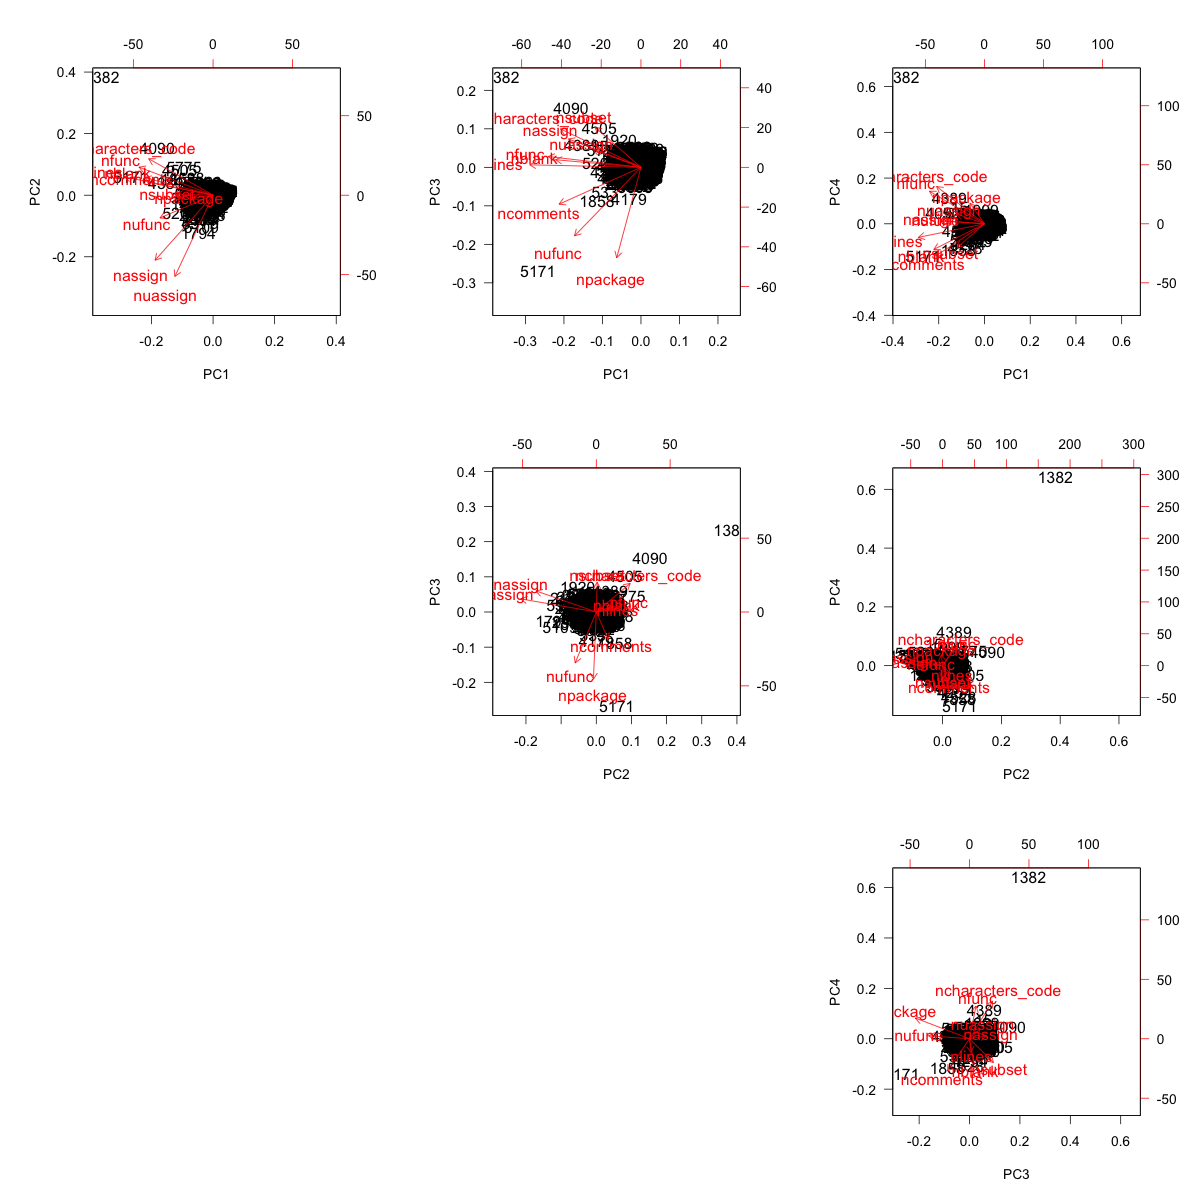
\includegraphics[width=16cm,height=16cm]{biplots}
\caption{Biplots for the first 4 principal components}
\end{figure}



% \bibliographystyle{chicago}
% \bibliographystyle{ieeetr}
% \bibliography{ref}

\end{document}


